\section{Experimental setup}
\label{sec:Experimental setup}

The experiment consits of a single scintillating fiber, which can be excited using a LED.
A picure of the setup can be ssen in \autoref{fig:exp}

\begin{figure}[H]
	\centering
	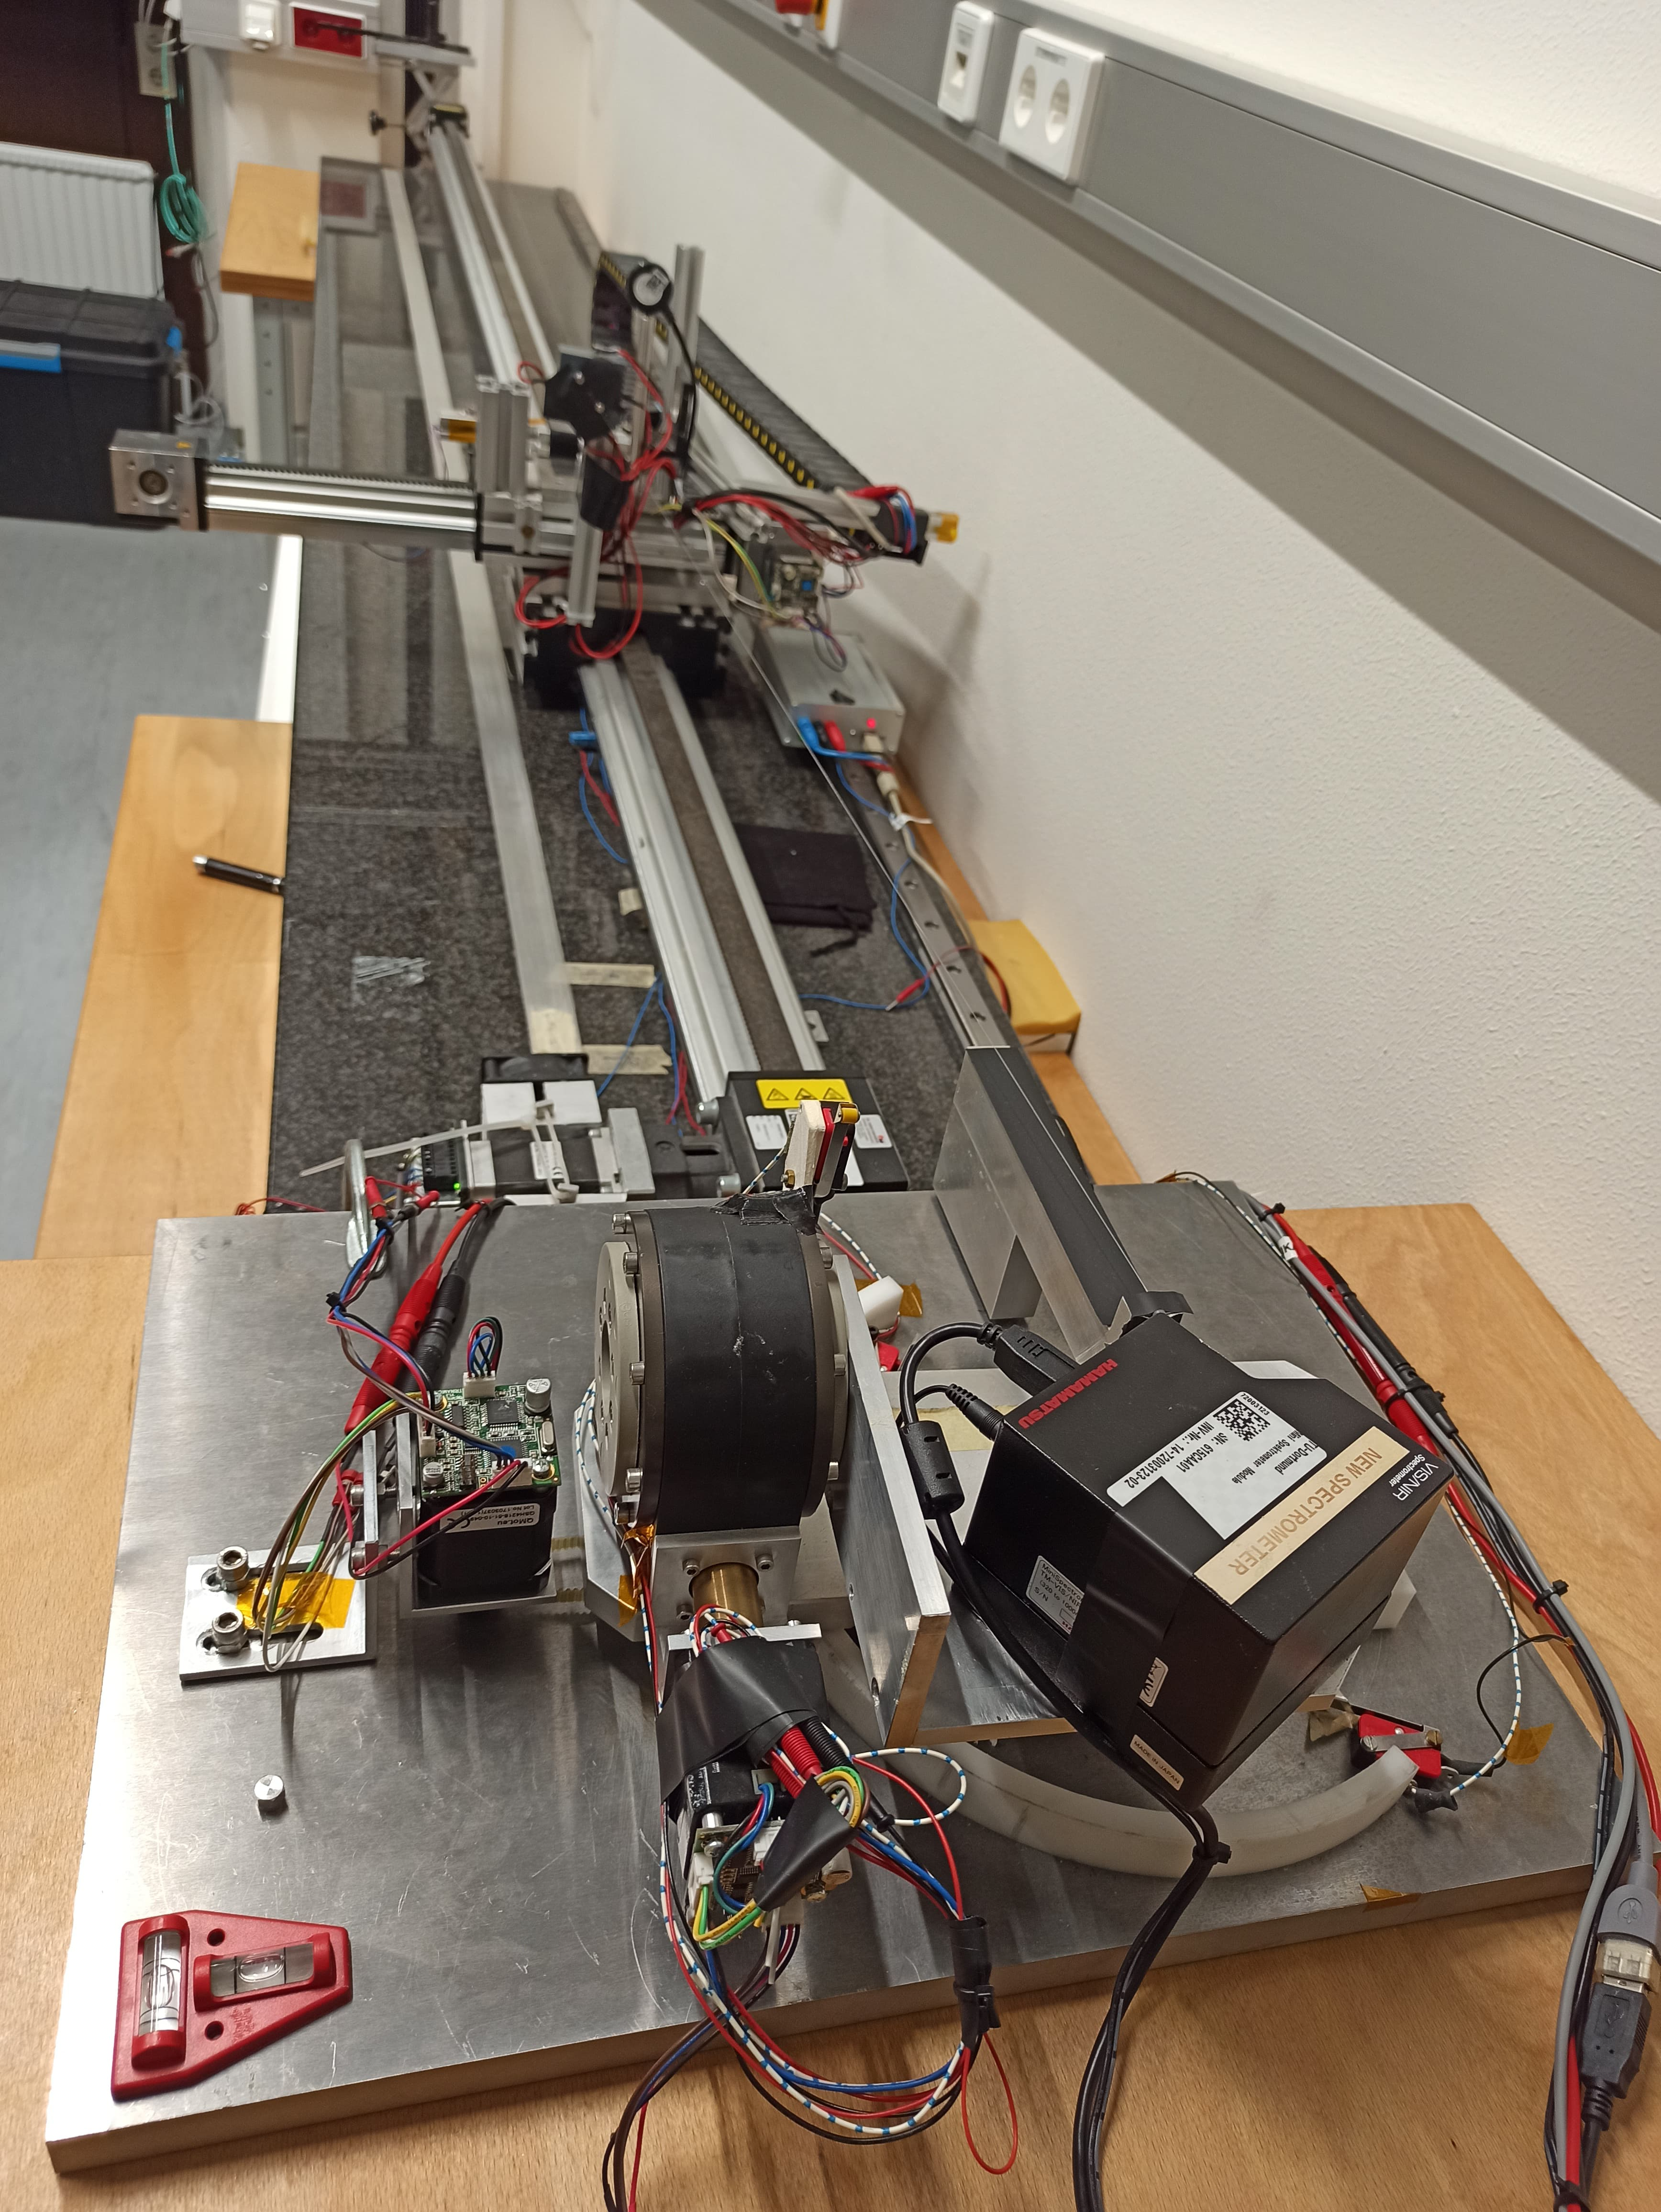
\includegraphics[width=0.5\linewidth]{pics/setup.jpg}
	\caption{Experimental setup consisting of the fiber, the LED and spectrometer.}
	\label{fig:exp}
\end{figure}

The LED can be moved along the fiber to be able to excite it at different positions. At one end of the fiber,
a spectrometer is positioned. It can be tilted in the horizontal and vertical plane in the angle intervals [-20°,90°]
and [-6°,90°], respectively.
The entire setup is connected to a computer, which runs a programm that allows to set all paramters for a measurement.
The simulation data needed for the analysis is already produced with \texttt{Geant4}. Here, 50 fibres were excited and simulated at 24 points each.
The resulting Monte Carlo data is transferred via USB-Stick to be analysed later.

\section{Measuring tasks}
\label{sec:Measuring tasks}

For every measurement, the dark counts are also saved. These are the counts that are measured by the spectrometer even
if the LED is turned of and the fiber is not excited. In the analysis, these will be substracted from the actual counts
to remove the effect of the dark current.
The current of the LED is always set to \qty{20}{\milli\ampere}. The same holds for the integration time and number of
averages, that are \qty{10000}{\micro\second} and \qty{5}{} in all measurements, respectively.

\subsection{Spectrometer measurement}
The first measurement is taken without varying the excitation position or the spectrometer angle. Instead, the wavelength
dependance of the emmited photons is measured by the spectrometer. This is done with the room light on and room light off,
the two results are later compared.

\subsection{Radial symmetry}
Now, the horizontal and vertical angle of the spectrometer are varied, while the excitation position is kept constant.
The angles intervall tested is [-18°,30°] in the horizontal plane and [-6°,35°] in the vertical plane. In both cases,
15 values are taken, resulting in a total of $225$ data points.

\subsection{Intensity measurement}
The dependancy of the light intensity on the distance is measured by altering the excitation location of the fibre.
The fiber is excited in an interval of \qty{150}{\centi\meter}, where the LED is moved in \qty{7.5}{\centi\meter}
increments. For each LED position, 10 different horizontal angles in the interval [0°,40°] are measured.
A defective spot in the fibre was visible when exciting it, its effect will be taken into account during the analysis.

\subsection{Angle Intensity measurement}
For the last measurement, the excitation position is kept constant again. The fiber is excited and only the
horizontal position of the spectrometer is varied in the interval [0°,45°]. 90 data points are taken by choosing
\qty{0.5}{\degree} steps between the measurements.